\section{System Modeling}

This section models the Smart Event Reminder System (SERS) from three complementary viewpoints: behavioral interaction, lifecycle state progression, and structural class relationships. Together, these diagrams provide a concise but complete understanding of how the system responds to user actions, how an event changes over time, and how the core software components are organized. The diagrams also serve as a communication bridge between the requirements phase and the implementation phase, ensuring that the design remains consistent with the project objectives.

\subsection{Sequence Diagram: Event Creation Workflow}

\begin{figure}[htbp]
	\centering
	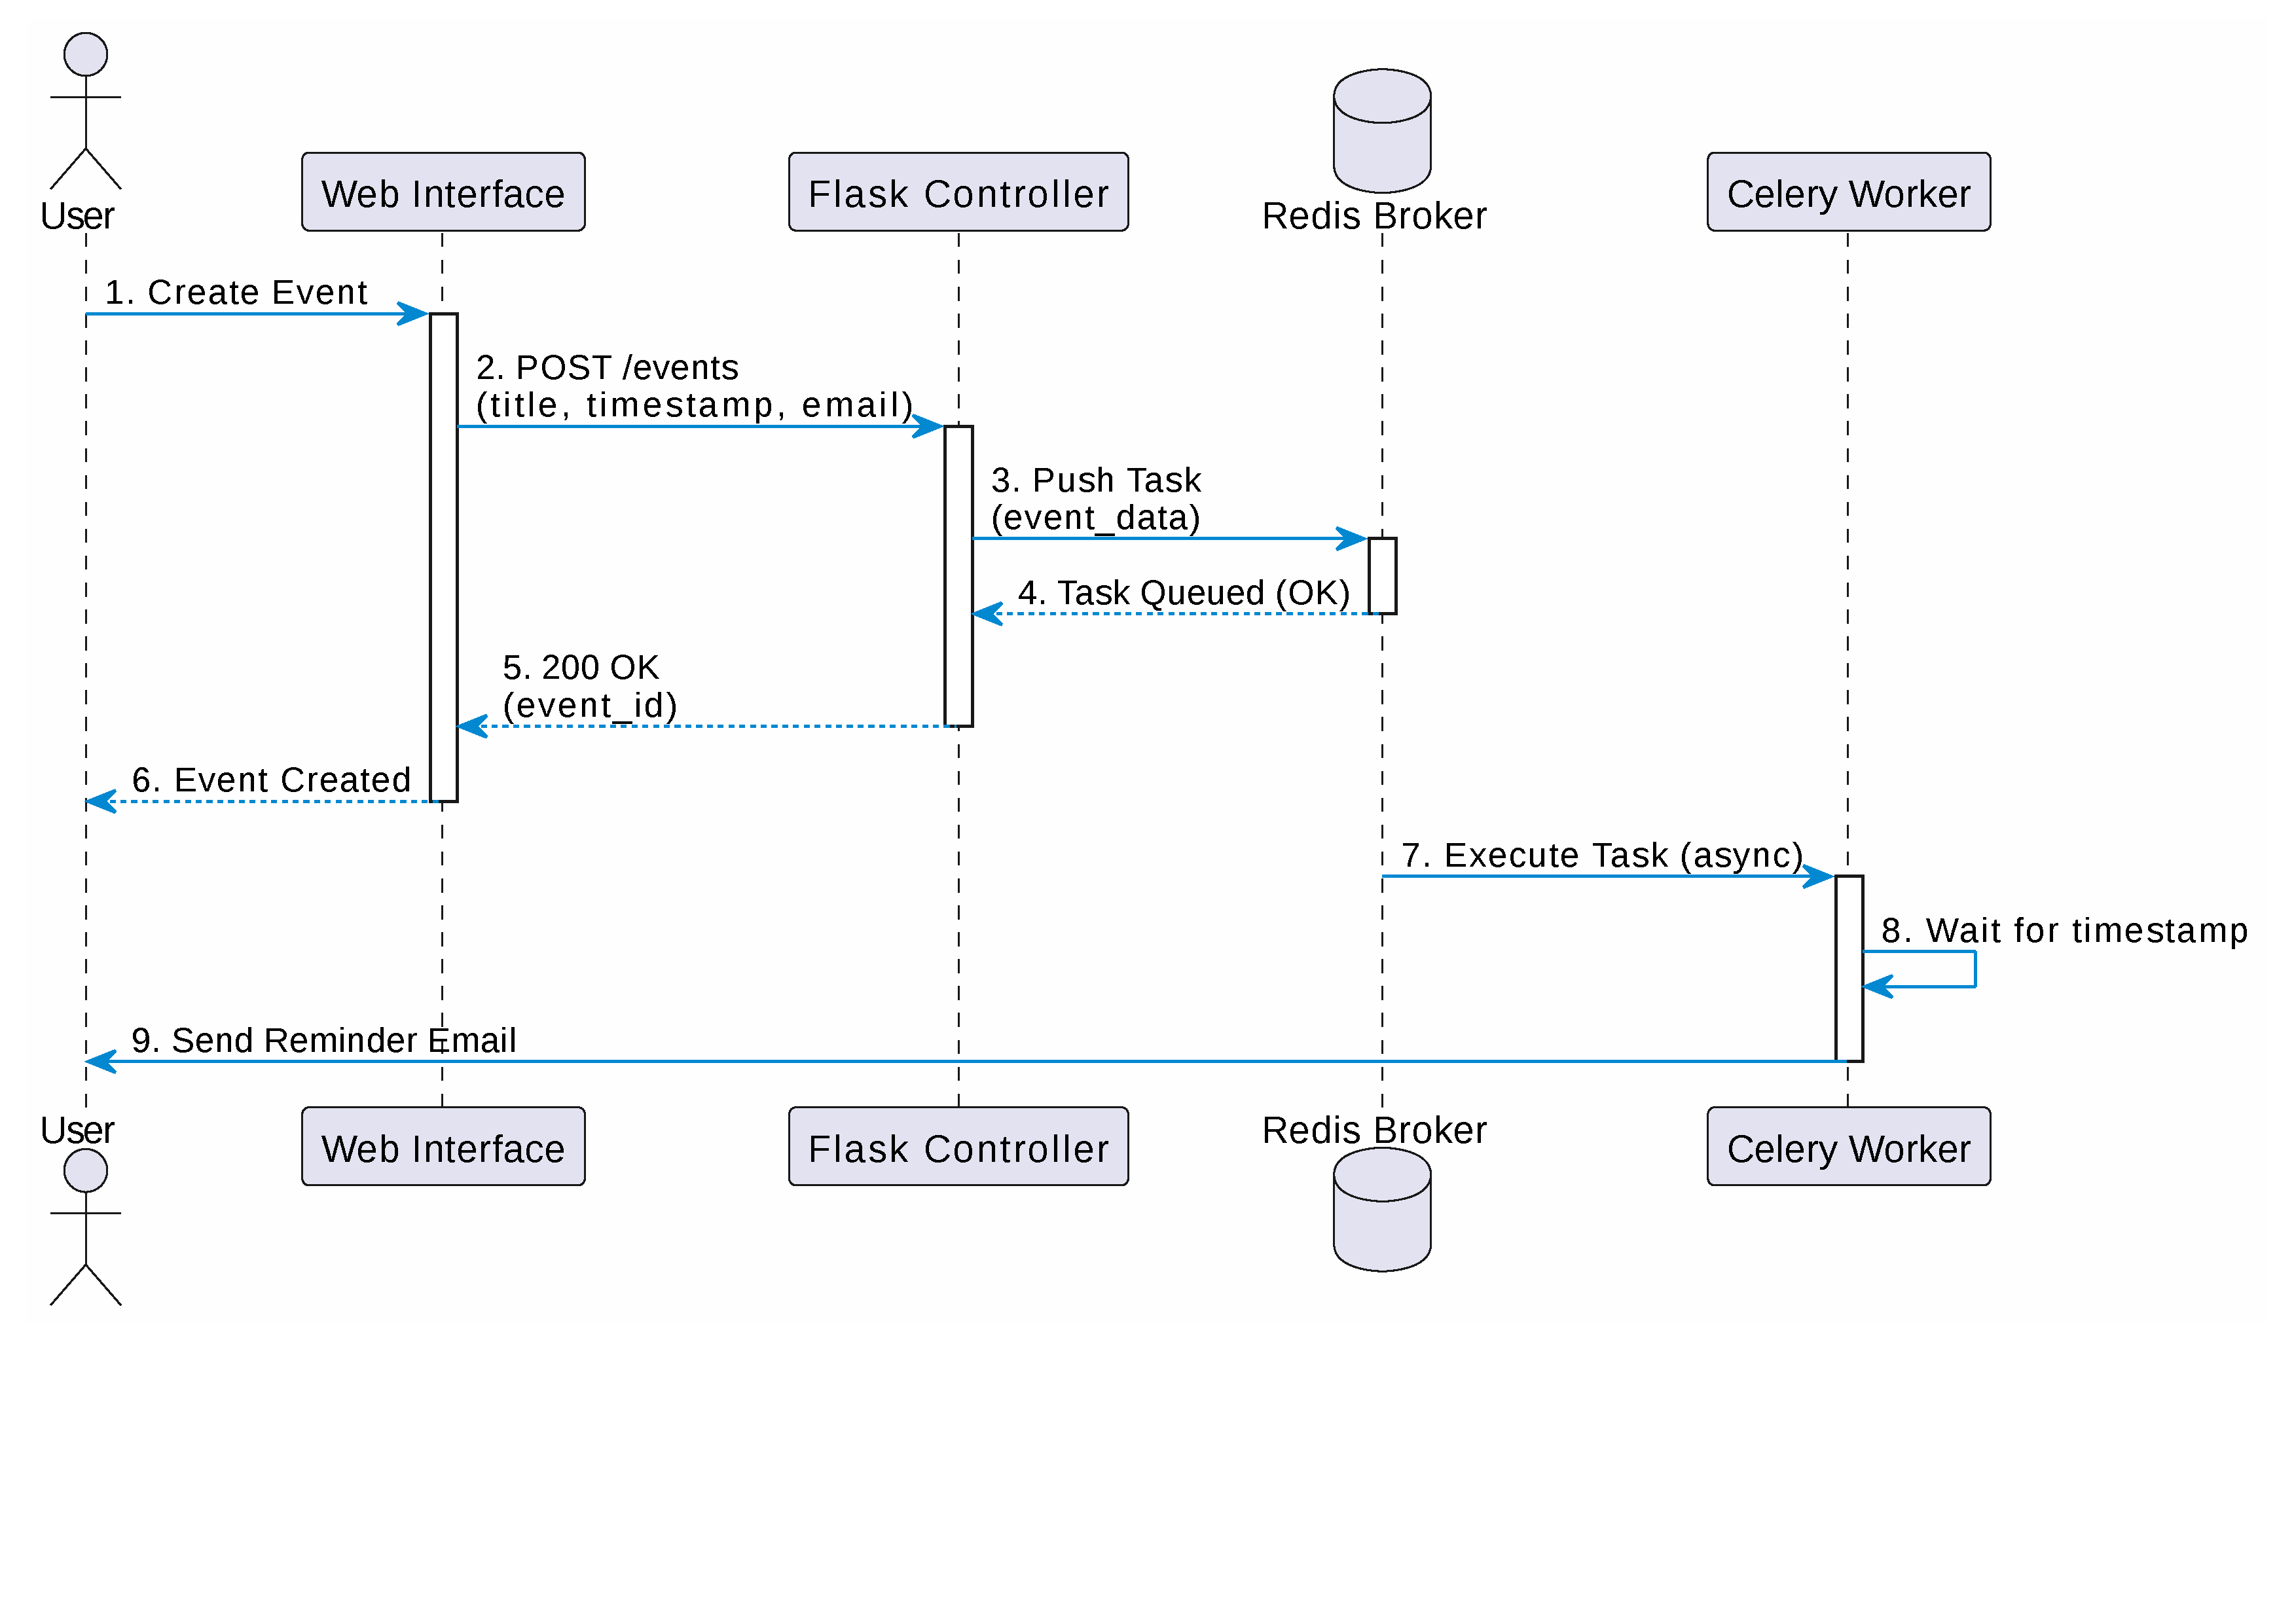
\includegraphics[width=\textwidth]{images/seq_diagram.pdf}
	\caption{Sequence diagram for creating a new event in SERS.}
	\label{fig:sequence-diagram}
\end{figure}

Figure~\ref{fig:sequence-diagram} illustrates the full interaction flow when a user creates a new reminder event. The sequence begins with the \textit{User} submitting a creation request through the \textit{Web Interface}. This request is then forwarded to the \textit{Flask Controller}, which acts as the central coordinator of the backend workflow. The controller validates the submitted data, such as the event title, timestamp, and target email address, before passing the event payload to the \textit{Redis Broker}. Redis is used as the message broker for scheduling asynchronous jobs, allowing the main application to remain responsive.

The diagram clearly separates synchronous and asynchronous communication. Steps 1 to 6 represent the immediate request-response cycle: the controller receives the request, queues the task, and returns an HTTP 200 OK response containing the generated event identifier. This confirms to the user that the event has been stored successfully without waiting for the reminder to be delivered. Steps 7 to 9 represent the asynchronous portion of the workflow, where the \textit{Celery Worker} independently monitors the queue, waits until the target time is reached, and finally sends the reminder notification. This design reflects the core principle of the system: the user interface should never block while background jobs are being processed.

From a software engineering perspective, this sequence diagram demonstrates the division of responsibilities across layers. The interface layer handles user interaction, the controller layer manages validation and orchestration, Redis handles task buffering, and Celery performs delayed execution. This arrangement supports scalability, fault isolation, and clean separation of concerns.

\subsection{State Diagram: Event Lifecycle}

\begin{figure}[htbp]
	\centering
	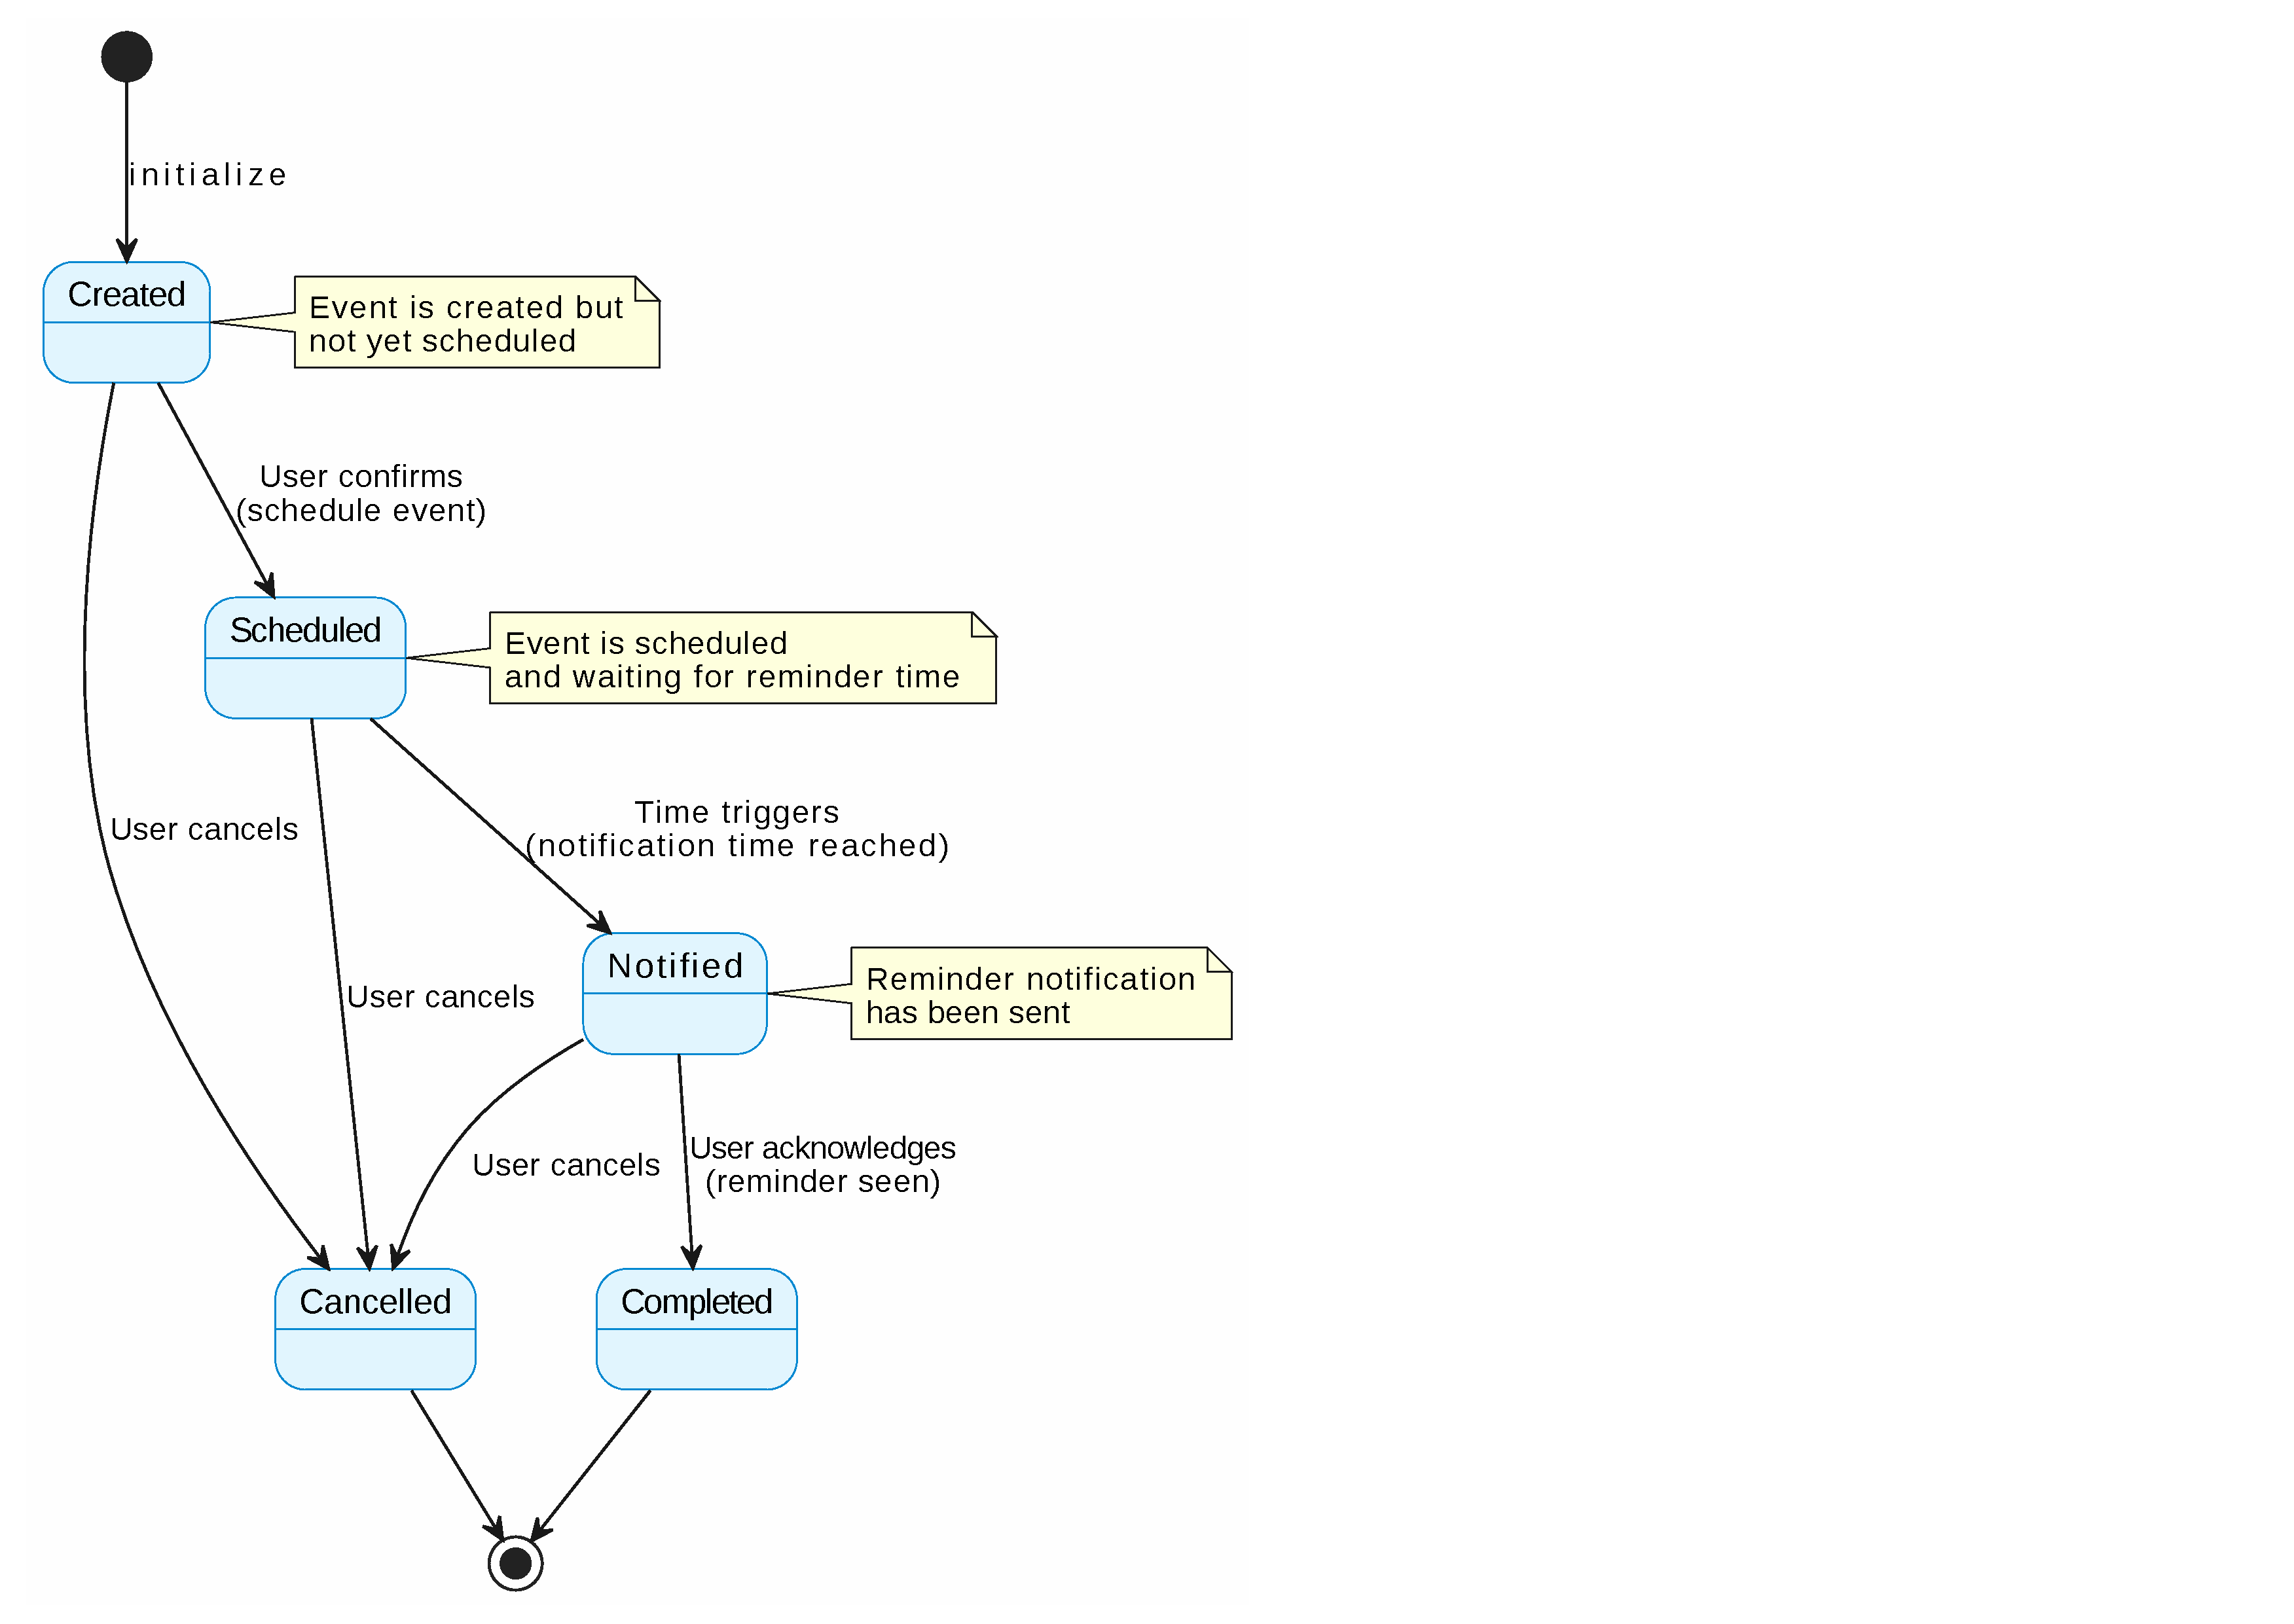
\includegraphics[width=0.88\textwidth]{images/state_diagram.pdf}
	\caption{State diagram showing the lifecycle of an event.}
	\label{fig:state-diagram}
\end{figure}

Figure~\ref{fig:state-diagram} presents the lifecycle of a single event as it moves through the system. The initial state is \textit{Created}, which represents an event that has been entered into the system but is not yet scheduled for execution. Once the user confirms the event details, the event transitions to \textit{Scheduled}. In this state, the reminder exists in the system and is waiting for the configured trigger time.

When the scheduled time is reached, the event moves to \textit{Notified}. This state indicates that the background worker has executed the reminder delivery process and the notification has been sent. After notification, the event may move to \textit{Completed} if the user acknowledges the reminder or the system records the workflow as finished. An alternative path exists through \textit{Cancelled}, which can be reached from either the \textit{Created}, \textit{Scheduled}, or \textit{Notified} states if the user decides to remove the event before it is finalized.

The diagram also emphasizes that cancellation is not a separate side case; it is an expected part of the event lifecycle. This is important for a reminder system because users frequently modify or delete events as schedules change. By modeling cancellation explicitly, the design remains faithful to real user behavior and avoids hidden assumptions about event completion.

\subsection{Class Diagram: Core Domain Structure}

\begin{figure}[htbp]
	\centering
	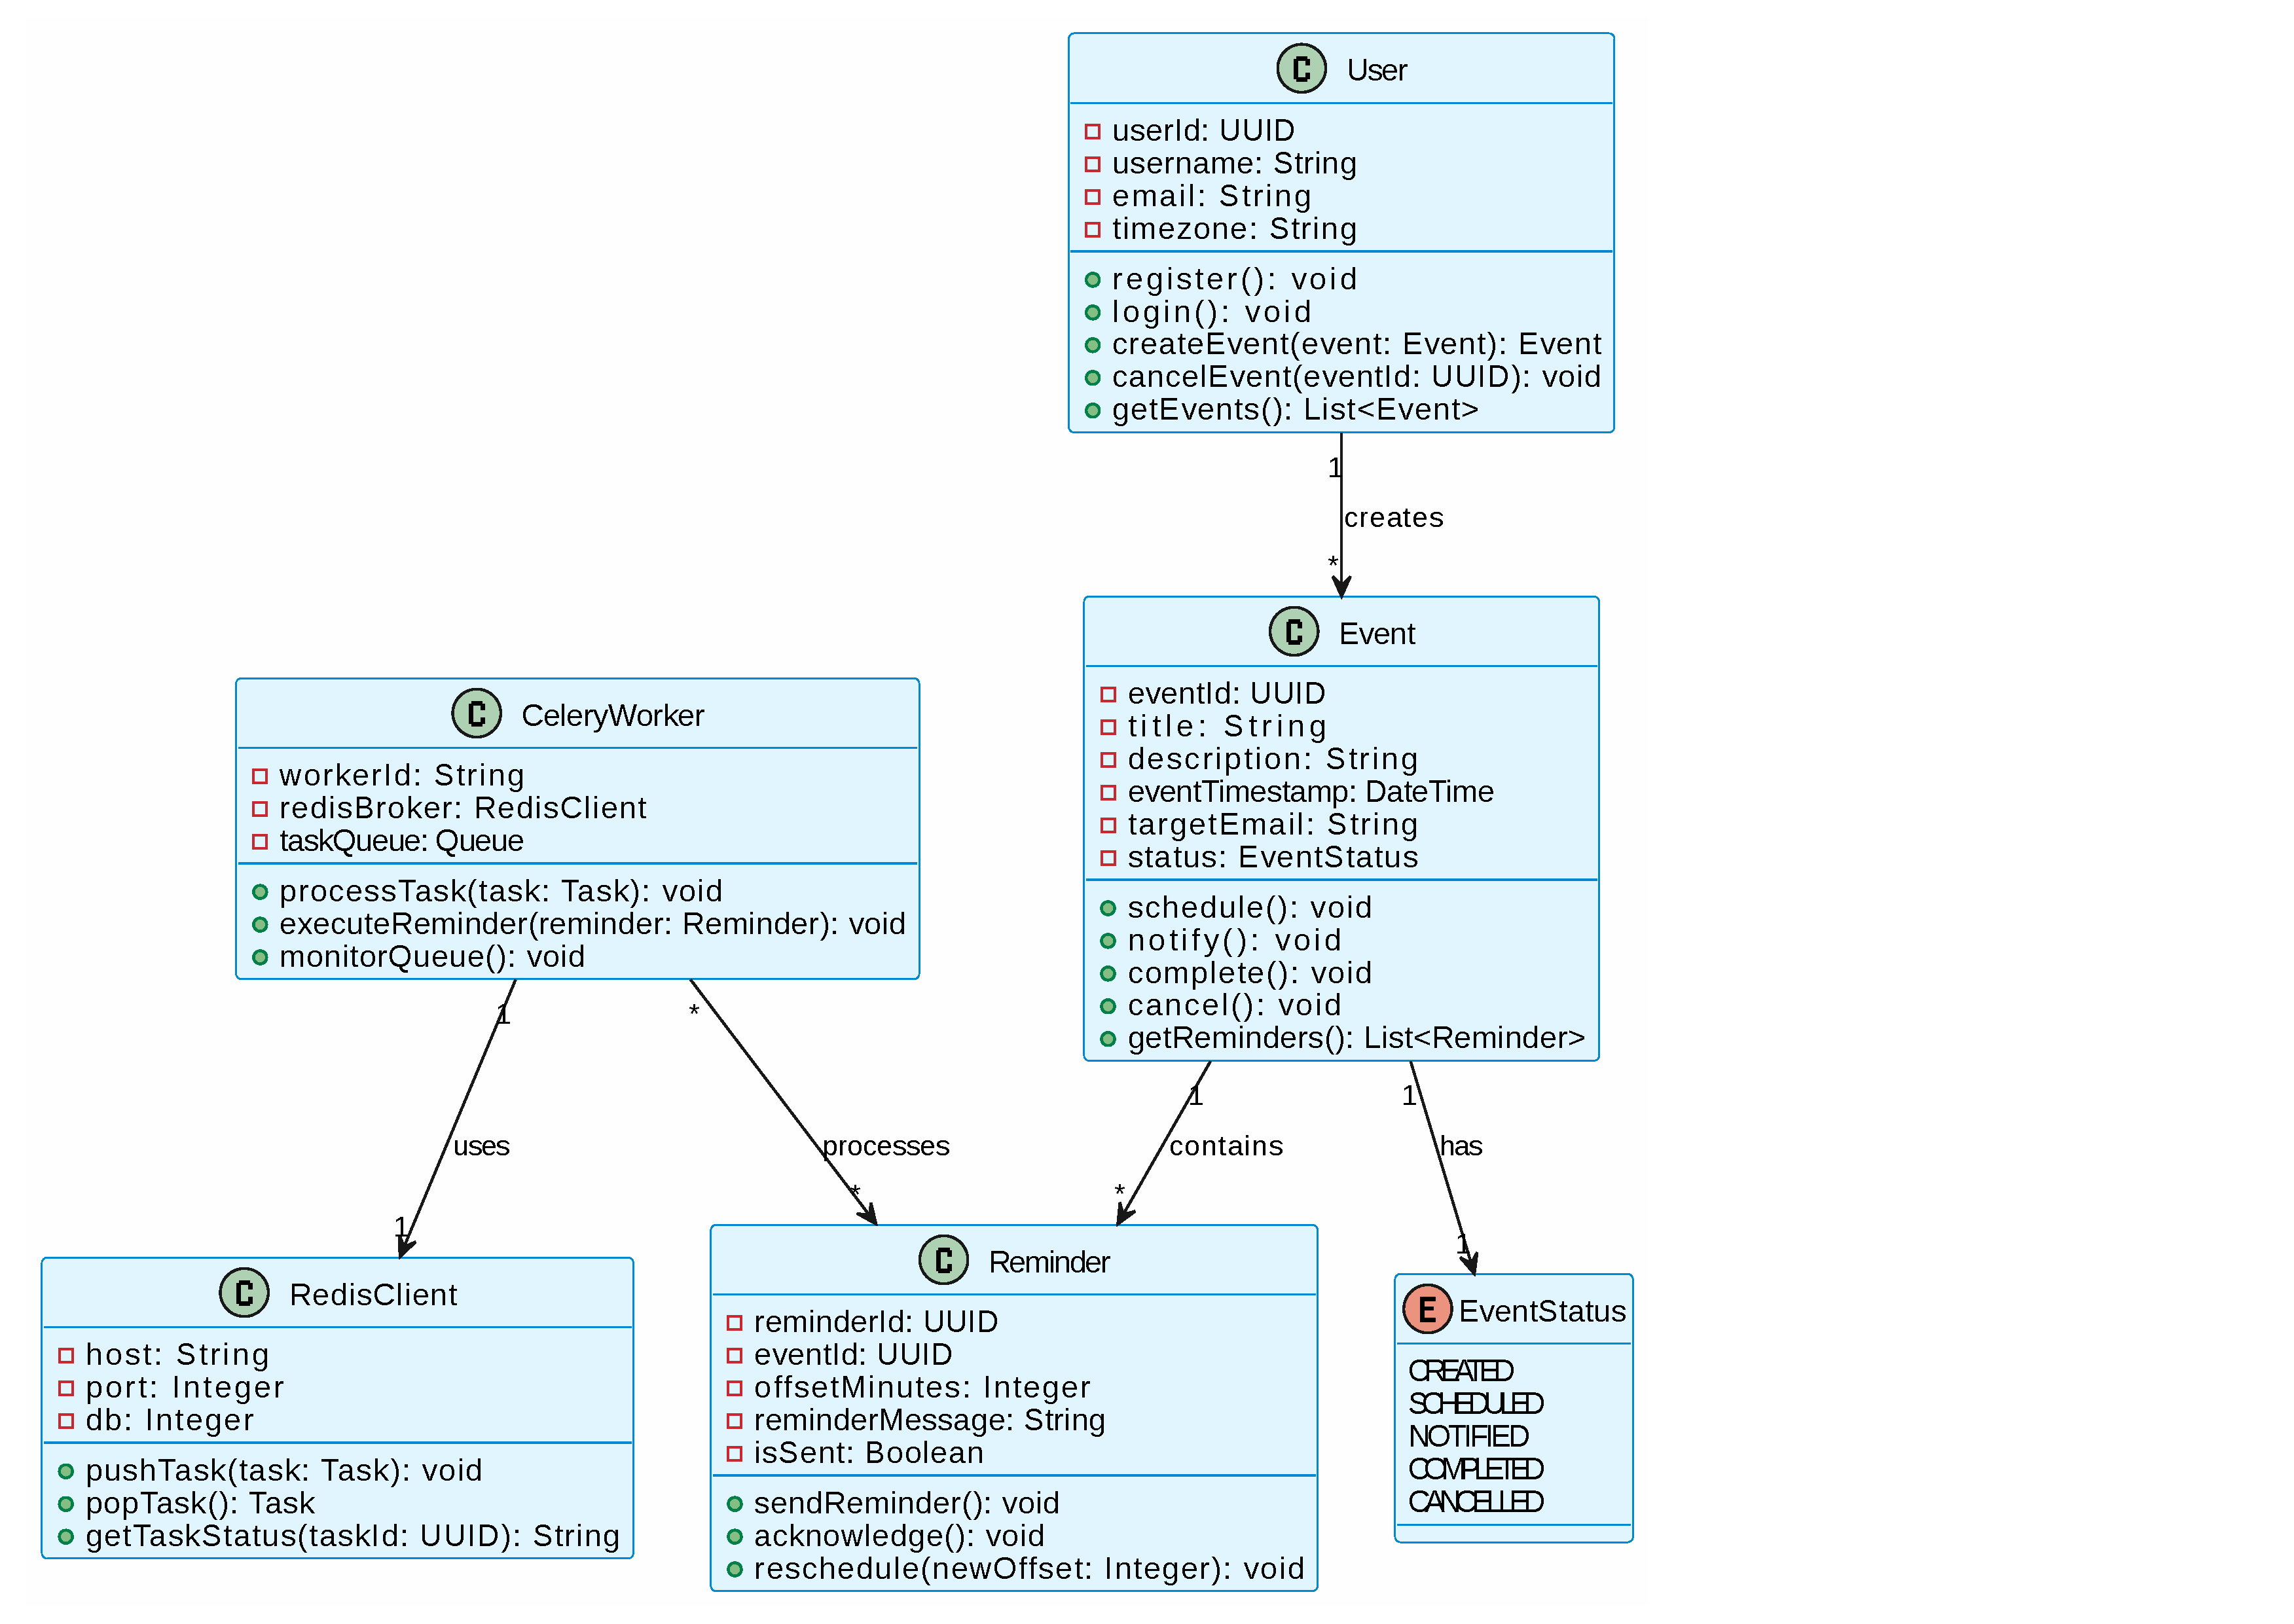
\includegraphics[width=\textwidth]{images/class_diagram.pdf}
	\caption{Class diagram for the main entities in SERS.}
	\label{fig:class-diagram}
\end{figure}

Figure~\ref{fig:class-diagram} describes the structural design of the system using the main domain classes. The \textit{User} class stores the basic identity information of a registered user and exposes operations such as registration, login, event creation, event cancellation, and event retrieval. The \textit{Event} class represents a scheduled reminder item and contains the key business data, including the title, description, timestamp, target email address, and current status. Its methods support the event lifecycle, such as scheduling, notifying, completing, and cancelling the event.

The \textit{Reminder} class captures reminder-specific data, such as the trigger offset, sent status, and associated event reference. Its operations support sending the reminder, acknowledging it, and rescheduling when necessary. The \textit{CeleryWorker} class models the asynchronous execution layer that processes reminder tasks independently from the web server. It interacts with the \textit{RedisClient} class, which represents the broker connection used to push and retrieve queued background jobs. Finally, the \textit{EventStatus} enumeration defines the valid lifecycle states for an event, ensuring that state transitions remain controlled and predictable.

This class diagram is especially useful because it maps the conceptual business rules to concrete software objects. It shows how the application separates persistent domain data from asynchronous processing infrastructure, and it makes the dependencies between components explicit. In practice, this helps the team implement the system consistently, reduces ambiguity during coding, and supports later maintenance or extension of the application.

\subsection{Summary}

Taken together, the three diagrams provide a complete model of the SERS application. The sequence diagram explains how a reminder is created and scheduled, the state diagram explains how an event evolves over time, and the class diagram explains how the system is structured internally. This combination of behavioral and structural modeling gives a clear design reference for implementation and testing.
